\chapter{System Design}
\label{ch:system-design}
\graphicspath{{./img/system-design/}}

In this section the block level system design is done and the direction-finding algorithm decided on.
The design is done based on the user requirements specified in \Cref{ch:introduction} as well as the data and background gathered in \Cref{ch:lit-review}.
Once the system is designed, some simulations are run to show whether the algorithm performs as expected and also to highlight potential problems that need to be tackled.

\section{Sub-systems}
The DF system will consist of the following sub-systems.
A block diagram view of what's been described here is shown in \Cref{fig:system-design:signal-flow} with some additional requirements noted.

\subsection{Antenna Array}
The antenna array will receive the RFI signals. The user requirements state that a \SI{360}{\degree} field of view is necessary. Hence, a circular array will be used. The arrays needs to be useful in direction-finding both narrowband and impulsive signals. This implies that a trade-off will have to be made in terms of element spacing when designing the array. If the element spacing is too large, the array will experience high amounts of phase ambiguity and perform poorly at narrowband DF. If the element spacing is too small the time difference for impulsive signals will be difficult to measure. The elements should be non-dispersive to facilitate keeping the structure of the impulsive signals. The number of elements to be used in the array will be explored later.

\subsection{Front End}
The front end will contain anti-aliasing filters and low noise amplifiers. For this project, a simple front end will be used. There will be no mixing or switching: the base band signal will be low pass filtered and amplified. The specifications of the filters and amplifiers will be specified based on the operating frequency band of the array and the sampling frequency of the ADCs. There will need to be an independent, identical RF chain for each element of the array.

\subsection{ROACH}
The ROACH board will have the functions of doing analogue to digital conversion and the high-speed digital signal processing. The ROACH consists of a Virtex 5 FPGA and multiple ADC cards allowing all of the RF inputs will be digitsed independently. The purpose of the ROACH is to do real-time processing on the raw ADC samples, hence reducing the data rate to only signals of interest which can be sent to the computer and processed there.

\subsection{Computer Software}
The computer will receive input from the ROACH and do further DSP. Specifically, the final angle of arrival estimation. The computer needs to be able to log all of the data for future analysis and display the results of the direction-finding to the user real-time in the field.


\begin{landscape}
  \thispagestyle{empty}
  \begin{figure}
    \centering
    \makebox[\textwidth][c] {
      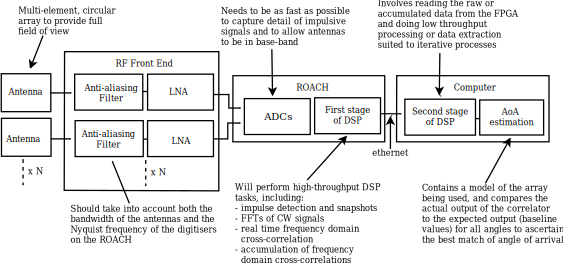
\includegraphics[width=\paperwidth]{basic-flow}
      % left, bottom, right, top
    }
  \caption{Block diagram view of the flow of signals through the proposed direction-finding system. The key function of the blocks has been noted on the diagram. }
  \label{fig:system-design:signal-flow}
  \end{figure}
\end{landscape}

\section{Direction Finding Algorithms}
With the above blocks in place, this section goes into selecting an appropriate direction-finding algorithm which meets user requirements and it refines what will be done in the first and second stage of DSP. Some additional requirements for the other blocks that arise from the selected algorithm are noted. 

This section details how the selected direction-finding algorithm will be implemented on the system. A simulation of the algorithm and the system in operation written in Python follows. The output of this simulation is shown, demonstrating that the algorithm is capable of carrying out the task.\\

There are two cases that the algorithm needs to deal with: weak narrowband signals and strong impulsive ones. The narrowband case naturally lends itself to frequency domain analysis since the information about narrowband continuous signals is concisely expressed in the frequency domain. The impulsive signals, however, are more naturally dealt with in the time domain as they are bound in time, existing only for a short duration, while being spread all over the frequency domain. 

As such, the selected algorithm contains two distinct parts: a phase interferometry component designed to direction-find weak (below the noise floor) narrowband signals, and a time difference of arrival part designed to locate short-duration impulsive RFI that are strong enough (ie: noticeable when plotted in the time domain).

\subsection{Phase Interferometry}
Phase Interferometry direction-finding of narrowband signals will be done by phase comparison of the signal of interest as seen by each element in the array. The technique of phase interferometry has been extensively explored in the literature review. The process carried out by this DF system will be the following steps:
\begin{enumerate}
  \item ADCs are used to sample the signal seen by each antenna exactly in phase. The ADCs need to be calibrated and have equal cable length to each antenna.
  \item The output of each ADC is streamed into a real-time FFT capable of producing Fourier transforms of the observed signals as fast as they are captured. Real-time implies that the FFTs must stream their frequency channel outputs at the same data rate as the rate which they they get in time domain data.
  \item Cross correlation between each pair of antennas is done to establish baselines. In the discrete frequency domain this means multiplying the value of each\footnote{It's not actually necessary to do each channel. If you know ahead of time the channel of interest the system need only accumulate that one, ignoring the rest. This reduces memory footprint, but means the entire spectrum cannot be read out and plotted or used for calibration, as well as making the system less dynamic/flexible.} frequency channel from one antenna by the complex conjugate of the value of the corresponding frequency channels from another antenna. The output of this complex conjugate multiplication is a spectrum where the phase of each channel is the phase difference of the two input spectra. The amplitude of the channel is simply the product of the two input amplitudes, but it's not that important for this application.
  \item Extract the signal of interest from the noise. For weak signals, the phase of the cross-correlation spectrum is corrupted by uncorrelated system noise. Attempting to read off phase difference from the output of a single FFT does not work as the phase would be dominated with noise. However, assuming we've got Gaussian white noise, the noise component should average to zero. Taking advantage of this we add multiple instances of these cross correlation spectra together. The signal component (observed phase difference difference of the signal seen by the baseline) sums coherently while the noise component sums to zero. As such, the more spectra are summed the more the signal component stands out from the noise.
  \item When sufficient baseline spectra have been summed, a snapshot of the result is taken and the phase of the channel of interest extracted from each baseline spectra. A \(M\)-dimensional vector of these observed baseline phase differences, where \(M = {N \choose 2}\) is the number of baselines.
  \item A \(M \times K\) matrix is constructed, representing the theoretical array response at various angles. Each column of the matrix is a vector of expected baseline phase shift for the AoA corresponding to that column. This is essentially a sampled antenna array manifold. Here \(K\) is the number of sample angles which the manifold is calculated for. It can be made as large as one wishes. A larger \(K\) means a higher resolution AoA estimation at the cost of more computational complexity.
  \item For each row in the calculated manifold matrix, the RMS error between the observed vector and that row is calculated. The column with the lowest RMS error is selected as the AoA of the signal. A measure of confidence can be given from the error.
\end{enumerate}

\subsection{Time Domain Direction Finding}
This technique is remarkably similar to phase interferometry. We are still capturing time domain signals from the antenna using ADCs that are sampling in phase to be able to measure a parameter of the received signal from the array. We are still comparing the value of the parameter to the theoretical response from the array at every angle in order to find the angle whose expected output most closely matches the observed signal. Hence much of the process described above will still apply.

The key difference is that instead of the parameter of interest being the phase difference of a frequency channel, the parameter of interest is the time difference of an impulsive signal at each antenna. As such it's necessary to capture time domain snapshots of the signals seen by each antenna and then do time domain cross-correlation to find the time domain offset of signals seen by each antenna. The peak of the cross-correlation output corresponds to the time difference.\footnote{Strictly speaking the peak offset is actually the ADC clock sample difference, but seeing as the ADC is being clocked at a known rate it can easily be converted to time difference. The antenna array manifold constructed will thus be in the time domain rather than the frequency domain.}

Additionally, as the time domain cross-correlation process is computationally expensive, it will only be done when a signal is detected. This implies that an impulse detector of some sort must be present and must be able to trigger the DF process.

\subsubsection{Upsampling for resolution}
For impulsive signals for which time domain DF will be used, there is no issue of ambiguity as such signal are not periodic, unlike continuous narrowband ones are. Instead, the issue is one of resolution. In order to get accurate time difference readings, a high time-resolution snapshot of the signals must be taken. The higher the time resolution of the signal, the more cross correlation points there are and the greater the accuracy of the time domain measurement. This means pushing the ADC faster.

Fortunately we can use upsampling to increase the resolution of the time domain cross-correlation provided that some requirements are met, and at the expense of additional computational complexity. The computational complexity comes both from the upsampling process as well as from the increased number of data points in the cross-correlation step.

The primary requirement is for a band-limited signal with no unwanted aliasing happening. The system designed here is doing base-band sampling which implies that this requirement is met provided a suitable low-pass filter is used in accordance with the Nyquist–Shannon sampling theorem. Sampling like this means that all of the information about the signal is captured in the samples. As the signal will thus be fully defined, smooth lines can be drawn between sampled points. This means that new higher resolution samples can be taken by interpolating more points (upsampling) between the sampled points.

This technique of upsampling is used to compensate for the fact that we'll be using a relatively small array, not typically suited to time domain direction-finding. A small array has a lower time-resolution which is good for limiting phase ambiguity for frequency domain direction-finding but produces unusably low time domain resolution unless upsampled.

\section{Algorithm Simulations}
\subsection{Frequency Domain Simulations}
In preparation for the implementation of the direction finding algorithms, a Python package called \lstinline{DirectionFinder_backend}\footnote{\url{https://github.com/jgowans/directionFinder\_backend}} is first written. This package has the code for an \lstinline{AntennaArray} class which builds an array model from arbitrary \lstinline{Antenna} objects. It can calculate and return a vector of the antenna array manifold for any given \lstinline{AntennaArray} and required number of sample points. The structure of this key package is discussed in more detail in \Cref{ch:software-design}.

An additional package, \lstinline{PhaseAmbiguity}\footnote{\url{https://github.com/jgowans/phase\_ambiguity}} is written containing scripts for creating an \lstinline{AntennaArray} object and then correlating the manifold vector from a reference direction to manifold vectors from all directions to find matches and plot the results. What this is doing in practice is assuming that the signal is actually coming from the given reference angle, \(\theta_{ref}\), and checking how similar (aka: ambiguous) a signal from another comparison angle, \(\theta_{comp}\), looks for a range of comparison angles.

The \lstinline{PhaseAmbiguity} simulator takes in as runtime arguments these parameters of frequency range, number of discrete frequency points, comparison AoA range, number of angle sample points points and the reference angle.
This produces a 3-D plot with axes for frequency, comparison angle and RMS error. Typically the 3-D plot is flattened to a 2-D image with colour used for the third dimension, rather than rendering a 3-D image. The type of data being plotted naturally lends itself to a colour plot view.

Ideally we would like 4-dimensional output: frequency, reference angle, comparison angle and correlation difference. However, this is difficult to visualise. Hence, two simulation approaches are used:
\begin{enumerate}
  \item fix reference angle while varying frequency and comparison angle, or
  \item fix frequency while vary reference and comparison angle.
\end{enumerate}
These different approaches produce results with a different view on the data. One view shows a slice of the ambiguity performance over a range of frequencies when the RFI emitter is located in a set direction. The other shows the ambiguity performance at a set frequency for a range of source locations. The combination of the two views gives a more complete picture of the ambiguity of the system for different parameters.

\subsection{Ambiguity Simulation Results}
The plots in \Cref{fig:system-design-phase-ambiguity-simulations} are of array ambiguity for antenna arrays ranging from 3 to 9 elements. As the number of elements increases the array radius is increased linearly to ensure equal spacing between elements is maintained.

The simulation is for a reference signal arriving from \SI{0}{\degree}, and comparing how similar signals from other angles appear to the system. This is a theoretical performance for a signal in no noise. The ideal performance is that all signals from all angles other than \SI{0}{\degree} have a distinguishable phase difference. Two observations are made:
\begin{enumerate}
  \item Arrays with an even number of elements suffer more from ambiguity than odd numbered arrays. This is due to there being line of symmetry in even numbered circular arrays. For example, a 4-element uniformly sampled circular array is actually a square.
  \item In general, the more elements you have, the lower the ambiguity. This is due to more baselines being able to resolve ambiguity.
\end{enumerate}

The plots in \Cref{fig:system-design:4-vs-5-element-fixed-baseline} show two examples of the other view of the data for 4 and 5 element arrays. Here both \(\theta_{ref}\) and \(\theta_{comp}\) are varied while \(f\) is fixed. The following observations are made:
\begin{enumerate}
  \item The 4 element array has points of true ambiguity where the signal arriving from \(\theta_{ref}\) and \(\theta_{comp}\) are mathematically identical even though the angles are different. The 5 element array does not have true ambiguity.
  \item Although no true ambiguity, the 5 element arrays does have bands of angles there the observed signals look more similar than other bands. Hence some angles are ``more ambiguous'' than others, meaning that it requires less noise or measurement error to throw off the result. This implies that the performance of the array is not exactly uniform. The reason for this is that the array is not a true circle, it's a sampled circled with 5 sample points. More sample points will reduce the contrast of these bands and make performance more uniform.
  \item The location of the bands of increased ambiguity is a function of the radius of the array measured in wavelengths. As such, the location of the bands will change with frequency.
\end{enumerate}

\begin{figure}[H]
  \centering
  \begin{subfigure}{0.95\textwidth}
    \centering
    \includegraphics[width=\textwidth, clip=true, trim = 10 15 53 0]{ambiguity03}
    % left, bottom, right, top
  \end{subfigure}\\[1em]
  \begin{subfigure}{\textwidth}
    \centering
    \includegraphics[width=\textwidth, clip=true, trim = 10 15 53 0]{ambiguity04}
  \end{subfigure}\\[1em]
  \begin{subfigure}{\textwidth}
    \centering
    \includegraphics[width=\textwidth, clip=true, trim = 10 15 53 0]{ambiguity05}
  \end{subfigure}
  \caption{Ambiguity plots for various array sizes with the reference signal arriving at \SI{0}{\degree}.}
  \label{fig:system-design-phase-ambiguity-simulations}
\end{figure}
\begin{figure}[H]
  \ContinuedFloat
  \centering
  \begin{subfigure}{0.95\textwidth}
    \centering
    \includegraphics[width=\textwidth, clip=true, trim = 10 15 53 0]{ambiguity06}
    % left, bottom, right, top
  \end{subfigure}\\[1em]
  \begin{subfigure}{\textwidth}
    \centering
    \includegraphics[width=\textwidth, clip=true, trim = 10 15 53 0]{ambiguity07}
  \end{subfigure}\\[1em]
  \begin{subfigure}{\textwidth}
    \centering
    \includegraphics[width=\textwidth, clip=true, trim = 10 15 53 0]{ambiguity09}
  \end{subfigure}
  \caption{(cont'd) Ambiguity plots for various array sizes with the reference signal arriving at \SI{0}{\degree}.}
\end{figure}

\begin{figure}[H]
  \centering
  \includegraphics[width=0.8\textwidth]{4element-fixedbaseline}
  \includegraphics[width=0.8\textwidth]{5element-fixedbaseline}
  \caption{Ambiguity simulation for a 4 element (top) and 5 element (bottom) array. The simulation is for a fixed frequency / baseline length, with variables for the true angle of arrival and a comparison angle, with output showing how different a signal from the comparison angle looks to the true angle. Ambiguity gets worse when the difference goes to zero. The 5 element array has better ambiguity performance due to no lines of symmetry.}
  \label{fig:system-design:4-vs-5-element-fixed-baseline}
\end{figure}


\subsubsection{Accumulation Gain Simulation Results}

\begin{figure}
  \centering
  \includegraphics[width=0.9\textwidth]{integration-vs-error-combined-5}
  \caption{Number of accumulations (aka: integrations) vs output error for various input SNR levels. It can be seen that accumulation decreases the error, and the decrease in error is faster for stronger signals.}
  \label{fig:system-design-integration-vs-error}
\end{figure}

The other performance criterion of the frequency domain system is an ability to see weak signals below the noise floor. The contention is that by accumulating many data points, the noise component will sum to zero while the signal component will sum coherently.

To verify this, the simulation package is extended to add coherent signals in the presence of white noise at configurable SNR levels. The coherent signal has a defined frequency and phase, and snapshots of 2048 samples of it are added to 2048 samples of white noise. The result is Fourier transformed and the phase of the signal of interest read off of the spectrum. The phase readings are accumulated as more and most snapshots are generated and measured. Phase error is measured after every snapshot / accumulation. The result is show in \Cref{fig:system-design-integration-vs-error}. This demonstrates that the more data points are accumulated, the more the real signal stands out of the noise. It also shows that the higher the SNR, the faster the error drops off. 

The structure of the simulation included many of the true limitations of the real system in order to make the result as meaningful as possible. This includes quantizing the input signal to 8-bits after being generated to simulate an ADC, as well as quantizing the output of the FFT to 32 bits to simulate the data bus widths that will be used in the FPGA.\\

This figure also demonstrates why it is difficult to quantify the performance of a DF system with a single ``accuracy'' number: the error is dependant on many factors, such as number of antenna elements, RFI signal strength and observation time.

\subsection{Time Domain Simulations}
\begin{figure}
  \centering
  \includegraphics[width=0.9\textwidth]{time-domain-cross-raw-vs-upped}
  \caption{Original cross correlation output with upsampled version overlaid. The upsampled version has a more accurate peak}
  \label{fig:system-design-raw-vs-upsampled-timedomain}
\end{figure}
The time domain system does not need either ambiguity or accumulations length simulations. The reason is that time domain DF of impulsive signals does not suffer from ambiguity, and accumulation is not done for impulsive signals. What it does do, however, is upsampling. To demonstrate this, a simulation of Fourier method upsampling is done here to show how it works. The Fourier method, also known as interpolation, involves taking the Fourier transform of the received impulsive signal, zero padding the DTFT output with \(L \times F\) zeros where \(L\) is the length of the observed signal in number of samples and \(F\) is the factor that the signal should be upsampled by. Next the inverse Fourier transform of the padded signal is done to get it  back to the time domain. It is legal to zero pad a Frequency domain signal provided the received signal does not have any out-of-band or aliased components. This can be ensured with good analogue filtering.

It is worth noting that this interpolation can be done either on the raw signals or equivalently on the output of the cross correlation. This is important as there will be significantly less computation involved in interpolating the output of the cross correlation than the raw time domain signals. The reason is that correlation is only done over a small window of the raw signal, not over the whole signal.\\

An example is shown in \Cref{fig:system-design-raw-vs-upsampled-timedomain}. Here, the red signal with few datapoints is the original output of the time domain cross correlation. There is a clear peak data point in red, however the data point to the left is higher, implying that the real, continuous signal's peak is probably more to the left of the observed peak. When an upsampling is done and plotted in blue, the peak of the interpolated signal is more what would be expected.

\section{Summary}
This chapter has discussed how a system with an antenna array, an RF front end, digitisers and DSP can be used to DF both narrowband and impulsive RFI. It's been shown how antenna geometry impacts ambiguity performance, how accumulation can allow us to see below the noise floor, and how interpolation can be used to increase resolution of a band limited signal.

TODO: add more to summary.
